\documentclass[10pt, a4paper]{article}
\usepackage[francais]{babel}
\usepackage[utf8]{inputenc}
\usepackage[T1]{fontenc}
\usepackage{hyperref}
\usepackage[]{graphicx}
\usepackage{url}
\usepackage[a4paper, left=2.5cm, right=2.5cm, top=2.0cm, bottom=2.0cm, headsep=1.0cm]{geometry}
\usepackage{subfigure}
\usepackage{epstopdf}
\usepackage{rotating}
\usepackage{wrapfig}

\setcounter{totalnumber}{5}
\renewcommand{\topfraction}{0.9}
\renewcommand{\bottomfraction}{0.9}
\newcommand{\linia}{\rule{\linewidth}{0.4mm}}

\renewcommand{\floatpagefraction}{0.7}

\newtheorem{mydef}{Definition}

\author{Yann Colin \\Grzegorz Maj}
\title{Médiatheque}

\makeatletter
\def\maketitle{%
\begin{titlepage}
	\begin{center}
		\LARGE
		\textsc{Compte rendu \\ Projet Informatique}
	\end{center}

	\vspace{3cm}

	\begin{center}\leavevmode
      \hrule
    \vskip 1pt
	\linia
	\vskip 0.5cm
	\Huge \textsc{\@title}\par

	\vskip 0.5cm
      	\linia
      \vskip 1pt
      \hrule

	\vskip 2mm

	\vspace{1.5cm}
	\begin{flushright}
		\begin{minipage}{5cm}
			\textit{\normalsize Auteurs:}\\
			\Large \textit{\@author} \par
			\vskip 2pt
			\hrule
			
		\end{minipage}
	\end{flushright}
    

	\end{center}%
	\vspace*{\stretch{6}}
    \begin{center}
    10 janvier 2016
    \end{center}
\end{titlepage}
	}
\makeatother



\begin{document}
\bibliographystyle{plain}
    \maketitle
    
    \tableofcontents
    \newpage
    
     \section{La conception}
     
	     \subsection{Diagramme de classes}
		\begin{figure}[ht]
	    \centering
	    		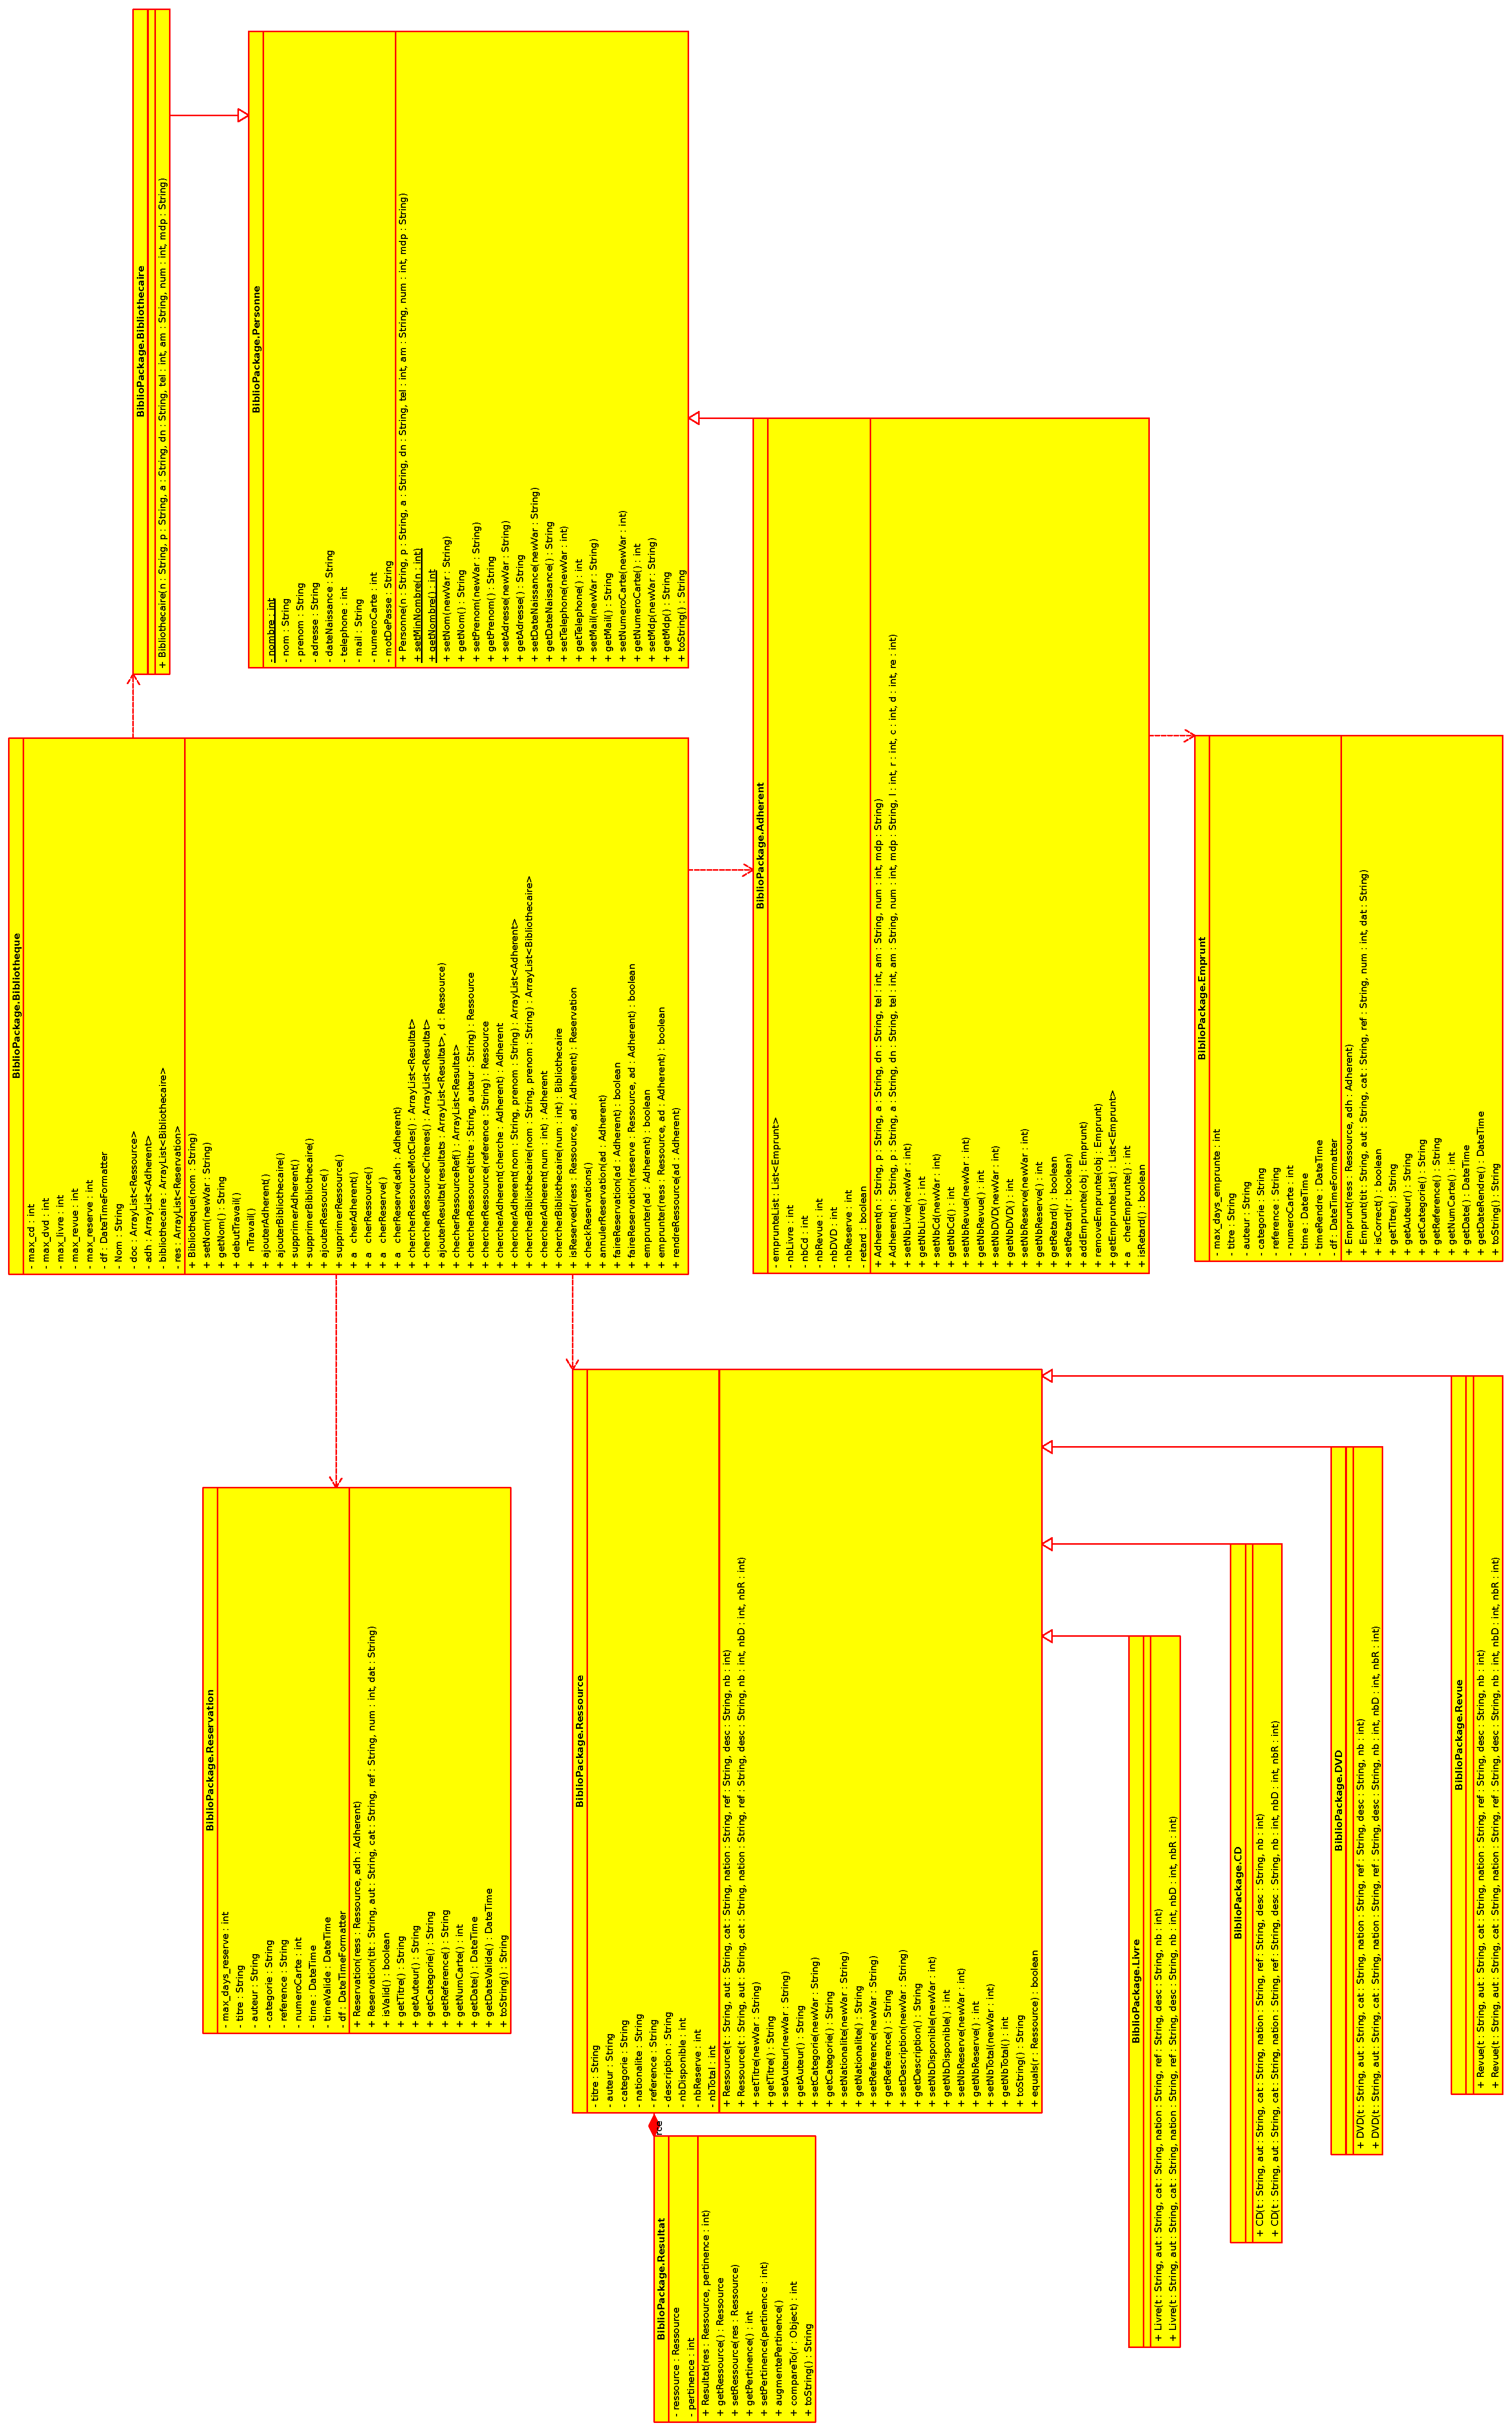
\includegraphics[width=0.7\textwidth]{graphics/class90.eps}
	    		\caption{Diagramme de classes}
	    		\label{fig:label}
	    	\end{figure}
	    	\newpage
     
    		 \subsection{Diagramme de cas d'utilisation}
    		 
    		 \begin{figure}[h]
			\begin{center}
				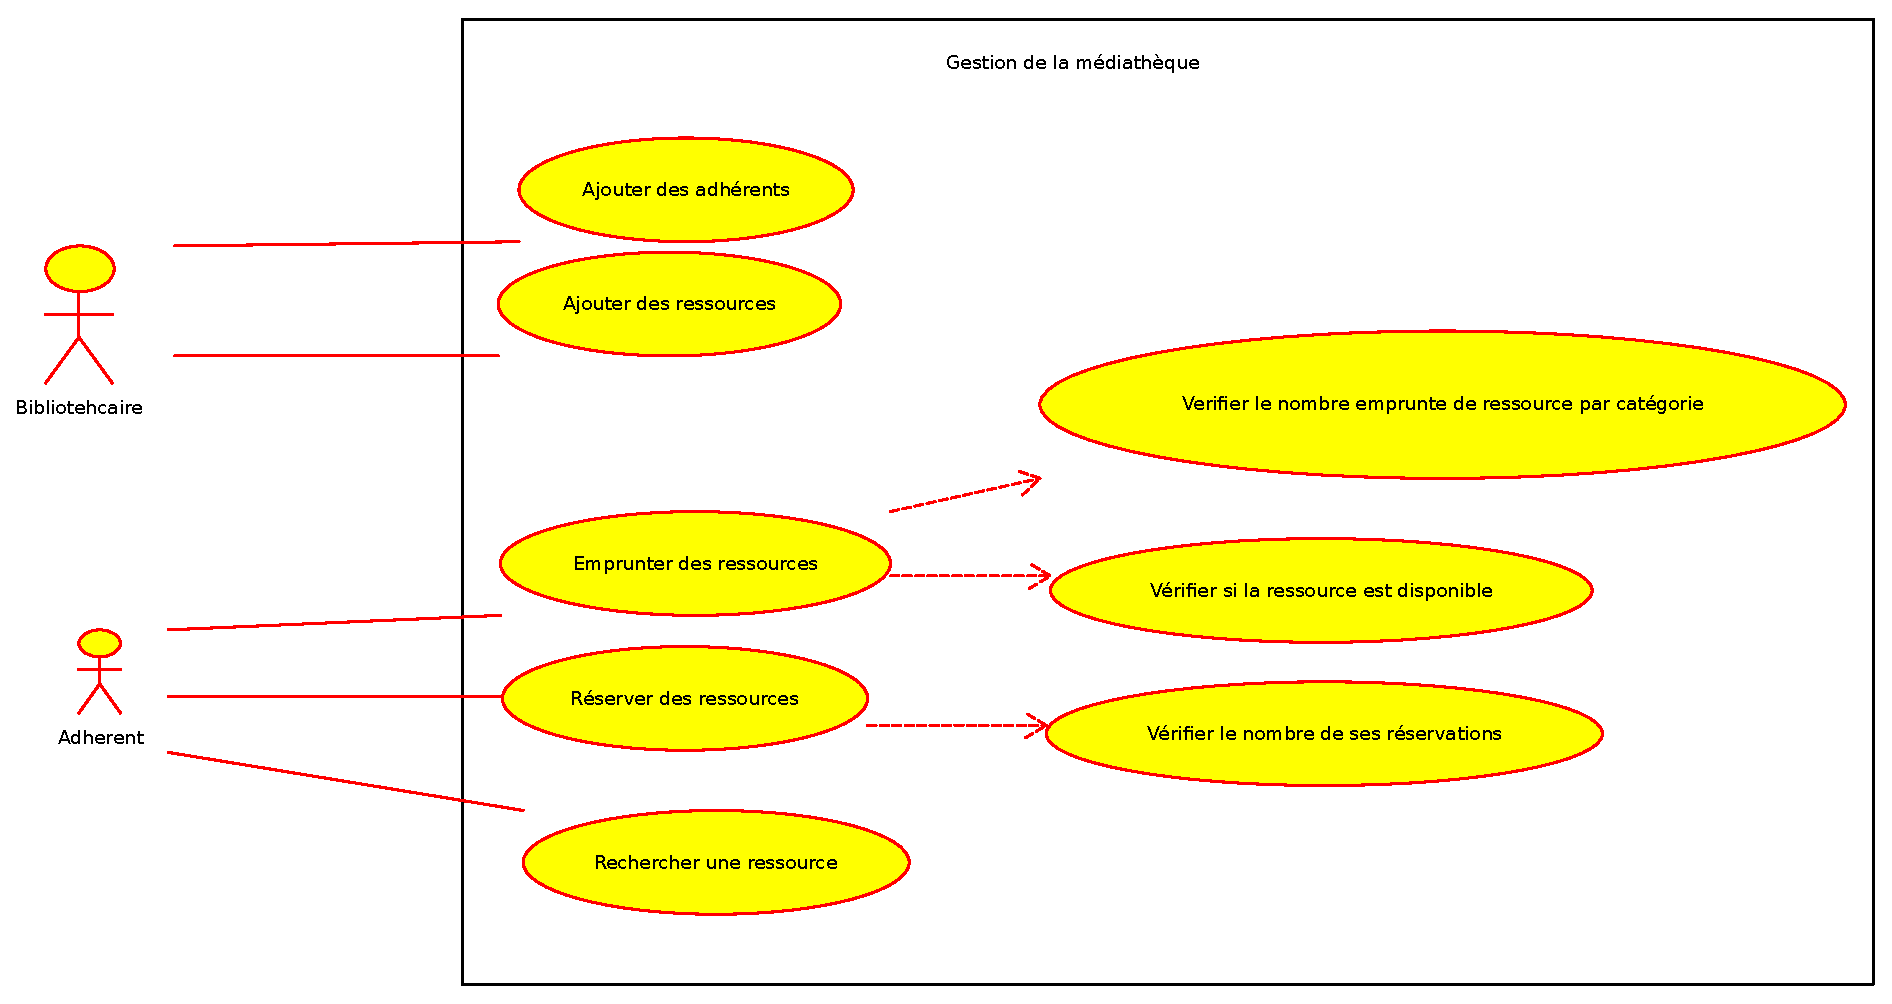
\includegraphics[width=1\textwidth]{graphics/usecasediagram.eps}
				\caption{Diagramme de cas d'utilisation.}
			\end{center}
		\end{figure}
	
	\section{Implémentation}
	Le logiciel est implémente dans la langue Java. Pour lire le commandes d'utilisateur on a utilise 
	la classe \texttt{Lire}.
	
	Le projet de mediatheque nécessite utiliser base de données ou enregistrer le données dans le fichier.
	On a considéré utilisation format XML ou JSON. On a choisi de JSON, parce que c'est plus léger et 
	simple que XML. Comme un parser on a choisi JSON.simple.
	
	Faire les emprunts et les réservations a besoin d'utiliser certain format de la date. On a utiliser 
	JodaTime qui est nouveau standard dans Java 8.
	
	\section{Les tests}
	Pendant les tests on a dû vérifier:
	\begin{enumerate}
		\item ajouter adhérent
		\item supprimer adhérent
		\item ajouter bibliothécaire
		\item supprimer bibliothécaire
		\item emprunter
		\begin{itemize}
			\item limites d'emprunt
			\item durée d'emprunt
		\end{itemize}
		\item rendre
		\item réservation
		\begin{itemize}
			\item limites de réservation
			\item durée de réservation
			\item annuler de réservation
		\end{itemize}
		\item la recherche de ressources 
	\end{enumerate}
	
	
	Le processus de vérification est inclus dans le fichier ....
	\section{Façon de travail}
		\subsection{Partage de travail}
		
		
		\subsection{Logiciel de gestion de version}
		Pendant le travail on a gardé tous les fichier sur na serveur GitHub avec utilisation du systeme 
		Git.
		
		\subsection{Les problèmes}
		
		
	

\bibliography{bibliografia.bib}

\end{document}
